\documentclass[12pt,a4paper]{report}

% ============================================================
% PACKAGES
% ============================================================

\usepackage[a4paper,
    left=1.25in,
    right=1.0in,
    top=1.0in,
    bottom=1.0in
]{geometry}

\usepackage{times}
\usepackage{setspace}
\usepackage{graphicx}
\usepackage{booktabs}
\usepackage{longtable}
\usepackage{array}
\usepackage{tabularx}
\usepackage{multirow}
\usepackage{enumitem}
\usepackage{float}
\usepackage{caption}
\usepackage{subcaption}
\usepackage{xcolor}
\usepackage{tikz}
\usepackage{amsmath}
\usepackage{amssymb}
\usepackage{url}
\usepackage{hyperref}
\usepackage{fancyhdr}
\usepackage{titlesec}
\usepackage{etoolbox}
\usepackage{ragged2e}
\usepackage{microtype}

\usetikzlibrary{
    positioning,
    arrows.meta,
    shapes.geometric,
    shapes.multipart,
    fit,
    backgrounds,
    calc
}

% ============================================================
% COLORS
% ============================================================

\definecolor{navy}{RGB}{25,45,75}
\definecolor{blue}{RGB}{40,90,150}
\definecolor{lightblue}{RGB}{225,235,248}
\definecolor{lightgray}{RGB}{242,242,242}
\definecolor{darkgray}{RGB}{80,80,80}
\definecolor{green}{RGB}{55,120,80}
\definecolor{orange}{RGB}{190,105,35}

% ============================================================
% HYPERLINK SETUP
% ============================================================

\hypersetup{
    colorlinks=true,
    linkcolor=navy,
    citecolor=blue,
    urlcolor=blue,
    pdftitle={Syllabus-Grounded Controllable Question Generation Using RAG and Lightweight LLMs},
    pdfauthor={Department of Computer Engineering}
}

% ============================================================
% PAGE STYLE
% ============================================================

\pagestyle{fancy}
\fancyhf{}

\fancyhead[L]{\small Syllabus-Grounded Controllable Question Generation}
\fancyhead[R]{\small Computer Engineering}

\fancyfoot[C]{\thepage}

\renewcommand{\headrulewidth}{0.4pt}
\renewcommand{\footrulewidth}{0pt}

% ============================================================
% CHAPTER STYLE
% ============================================================

\titleformat{\chapter}
    {\normalfont\Huge\bfseries\color{navy}}
    {Chapter \thechapter}
    {20pt}
    {}

\titleformat{\section}
    {\normalfont\Large\bfseries\color{navy}}
    {\thesection}
    {12pt}
    {}

\titleformat{\subsection}
    {\normalfont\large\bfseries\color{blue}}
    {\thesubsection}
    {10pt}
    {}

\setlength{\parindent}{0pt}
\setlength{\parskip}{7pt}

\onehalfspacing

% ============================================================
% TABLE SETTINGS
% ============================================================

\renewcommand{\arraystretch}{1.25}

\newcolumntype{Y}{>{\RaggedRight\arraybackslash}X}
\newcolumntype{P}[1]{>{\RaggedRight\arraybackslash}p{#1}}

% ============================================================
% CUSTOM COMMANDS
% ============================================================

\newcommand{\projecttitle}{
Syllabus-Grounded Controllable Question Generation\\
Using RAG and Lightweight LLMs
}

\newcommand{\university}{
University of Mumbai
}

\newcommand{\college}{
SHAH \& ANCHOR KUTCHHI ENGINEERING COLLEGE
}

\newcommand{\department}{
DEPARTMENT OF COMPUTER ENGINEERING
}

\newcommand{\academicyear}{
2026--2027
}

% ============================================================
% DOCUMENT
% ============================================================

\begin{document}
\begin{titlepage}
\begin{center}

\vspace*{0.2cm}

% Report heading
{\fontsize{20}{23}\selectfont \textbf{A}}\\[0.05cm]
{\fontsize{20}{23}\selectfont \textbf{REPORT}}\\[0.35cm]

% Degree statement
{\fontsize{11}{13}\selectfont
Submitted for Partial Fulfillment of the Requirement}\\[0.05cm]

{\fontsize{11}{13}\selectfont
for the award of the degree of}\\[0.20cm]

{\fontsize{15}{18}\selectfont
\textbf{BACHELOR OF TECHNOLOGY}}\\[0.18cm]

{\fontsize{11}{13}\selectfont in}\\[0.08cm]

{\fontsize{14}{17}\selectfont
\textbf{Computer Engineering}}\\[0.35cm]

% ON
{\fontsize{11}{13}\selectfont \textbf{ON}}\\[0.25cm]

% Project title
{\fontsize{17}{19}\selectfont
\textbf{\shortstack{
Syllabus-Grounded Controllable Question\\
Generation\\
Using RAG and Lightweight LLMs
}}
}\\[0.15cm]
% Submitted by
{\fontsize{11}{13}\selectfont \textbf{Submitted by}}\\[0.20cm]

{\fontsize{10.5}{13}\selectfont
\begin{tabular}{c}
\textbf{Dhruv Gala} \quad (23UF17719CM141)\\
\textbf{Yash Pajwani} \quad (23UF16586CM037)\\
\textbf{Shravan Padhar} \quad (23UF17927CM162)\\
\textbf{Sahil Shah} \quad (23UF17713CM049)
\end{tabular}
}

\vspace{0.25cm}

% College logo

\includegraphics[width=25mm]{SAKEC_logo.png}

\vspace{0.18cm}

% Guide
{\fontsize{11}{13}\selectfont
Under the guidance of}\\[0.10cm]

{\fontsize{11}{13}\selectfont
\textbf{Dr. Atul Haribhau Kachare}}\\[0.03cm]

{\fontsize{10}{12}\selectfont
Professor}

\vfill

% Department and college
{\fontsize{13}{15}\selectfont
\textbf{\department}}\\[0.10cm]

{\fontsize{11}{13}\selectfont
\textbf{\college}}\\[0.05cm]

{\fontsize{10}{12}\selectfont
(An Autonomous Institute Affiliated to University of Mumbai)}\\[0.08cm]

{\fontsize{10}{12}\selectfont
MUMBAI -- 400 088, MAHARASHTRA (INDIA)}\\[0.10cm]

{\fontsize{11}{13}\selectfont
\textbf{\academicyear}}

\end{center}
\end{titlepage}% ============================================================
% ABSTRACT
% ============================================================

\chapter*{ABSTRACT}
\addcontentsline{toc}{chapter}{Abstract}

Automatic question generation using Large Language Models has become increasingly capable, but directly prompting an LLM to generate educational questions does not guarantee that the generated questions remain aligned with a prescribed syllabus, cognitive level, difficulty, or question type. Questions may also contain factual hallucinations, repeated concepts, weak distractors, or content outside the intended curriculum.

This project proposes a \textbf{Syllabus-Grounded Controllable Question Generation System} based on Retrieval-Augmented Generation (RAG) and lightweight Large Language Models. The proposed system first processes and indexes educational resources such as textbooks, lecture notes, syllabus documents, and reference material. Given a question-generation request, the system retrieves relevant curriculum-grounded context before generating candidate questions.

The generation process is controlled through multiple constraints including \textbf{topic, difficulty, Bloom's taxonomy level, grounding requirements, question type, and diversity}. These constraints are jointly supplied to the generation controller rather than treating them as independent post-processing options. A lightweight locally deployable LLM is used to reduce computational and infrastructure requirements.

Generated questions subsequently pass through an automated validation pipeline. The validator checks syllabus relevance, factual grounding, Bloom-level alignment, difficulty, structural correctness, answer consistency, distractor quality, and semantic similarity against previously generated questions. Embedding-based diversity filtering is used to reduce repetitive questions.

The project therefore focuses not merely on generating questions, but on developing a controlled generation and validation pipeline capable of producing higher-quality, syllabus-aligned educational questions using affordable and privacy-preserving computational resources.

\textbf{Keywords:} Retrieval-Augmented Generation, RAG, Question Generation, Large Language Models, Bloom's Taxonomy, Educational AI, Syllabus Grounding, Semantic Similarity, Question Validation, Lightweight LLM.

% ============================================================
% CONTENTS
% ============================================================

\tableofcontents
\newpage

\listoffigures
\newpage

\listoftables
\newpage

% ============================================================
% CHAPTER 1
% ============================================================

\chapter{Introduction}

\section{Background}

Question generation is an important component of digital learning systems, assessment platforms, examination preparation systems, and educational content creation. Traditionally, educators manually create questions by studying prescribed textbooks, lecture notes, learning objectives, and previous examination patterns.

Although manual question creation provides strong curriculum control, it is time-consuming and difficult to scale. The emergence of Large Language Models (LLMs) has made automated question generation substantially easier. Modern LLMs can generate questions from a topic or a passage with minimal prompting.

However, simply generating a question using an LLM does not guarantee that the question satisfies educational requirements. A generated question may be technically correct but still be unsuitable because it tests the wrong cognitive skill, lies outside the prescribed syllabus, is too easy or too difficult, repeats an existing question, or contains ambiguous answer choices.

The problem therefore shifts from simple question generation to \textbf{controllable and verifiable question generation}.

\section{Limitations of Direct LLM-Based Question Generation}

A direct LLM prompting approach may exhibit several limitations:

\begin{enumerate}

\item \textbf{Syllabus mismatch:}
The model may generate questions using general knowledge that is not part of the prescribed curriculum.

\item \textbf{Weak Bloom's Taxonomy alignment:}
A question requested at an ``Analyze'' or ``Evaluate'' level may still become a simple recall or definition question.

\item \textbf{Difficulty instability:}
Difficulty instructions such as ``easy'', ``medium'', and ``hard'' are subjective and may not consistently control the resulting question.

\item \textbf{Hallucination:}
The model may generate technically plausible but unsupported facts.

\item \textbf{Question repetition:}
Generating several questions independently can result in semantically similar questions.

\item \textbf{Weak distractors:}
Multiple-choice questions may contain distractors that are obviously incorrect or unrelated to the concept.

\item \textbf{Poor scenario generation:}
Scenario-based questions may not adequately represent realistic application or analysis situations.

\end{enumerate}

\section{Motivation}

The motivation of this project is to build a system in which question generation is treated as a controlled pipeline rather than a single LLM prompt.

The proposed approach combines:

\begin{itemize}
    \item syllabus-grounded retrieval,
    \item controllable generation,
    \item lightweight LLM inference,
    \item automated question validation,
    \item semantic diversity filtering,
    \item Bloom's taxonomy control,
    \item difficulty control, and
    \item empirical evaluation through component-wise ablation.
\end{itemize}

This makes the system suitable for educational environments where both question quality and computational feasibility are important.

% ============================================================
% CHAPTER 2
% ============================================================

\chapter{Problem Identification}

\section{Existing Approach}

The simplest approach to automated question generation is:

\begin{center}
\textbf{Topic / Prompt $\rightarrow$ LLM $\rightarrow$ Questions}
\end{center}

Although this approach is easy to implement, it provides limited control over the educational properties of the generated questions.

A question generation system intended for academic use must consider multiple dimensions simultaneously.

\section{Identified Problems}

\subsection{Syllabus Grounding}

An LLM may possess information about a subject that extends beyond the prescribed syllabus. Therefore, general model knowledge cannot be treated as the authoritative source for curriculum-specific generation.

\subsection{Cognitive-Level Control}

Bloom's taxonomy provides a useful framework for describing cognitive complexity. The six commonly used levels are:

\begin{enumerate}
    \item Remember
    \item Understand
    \item Apply
    \item Analyze
    \item Evaluate
    \item Create
\end{enumerate}

A controllable question generator should be able to generate questions that correspond to the requested cognitive level.

\subsection{Difficulty Control}

Difficulty is influenced by several factors including conceptual complexity, number of reasoning steps, prerequisite knowledge, distractor similarity, and scenario complexity. A simple textual instruction such as ``generate a hard question'' does not guarantee consistent difficulty.

\subsection{Question Diversity}

Repeated questions reduce the usefulness of an automatically generated question bank. Two questions may use different wording while testing essentially the same concept.

Therefore, diversity must be evaluated semantically rather than only through exact string matching.

\subsection{Question Quality}

Generated questions require validation before being included in the final question bank. The validation process must identify:

\begin{itemize}
    \item factual inconsistencies,
    \item syllabus violations,
    \item incorrect answers,
    \item weak distractors,
    \item ambiguity,
    \item Bloom-level mismatch,
    \item difficulty mismatch, and
    \item excessive similarity to existing questions.
\end{itemize}

\section{Core Problem}

The core problem addressed by this project is:

\begin{quote}
\textit{How can a lightweight and locally deployable LLM be used with retrieval and automated validation to generate diverse, syllabus-grounded questions while providing explicit control over topic, difficulty, Bloom's cognitive level, and question type?}
\end{quote}

% ============================================================
% CHAPTER 3
% ============================================================

\chapter{Literature Survey \& Gap Analysis}

\section{Literature Survey}

Recent research has explored the use of LLMs, Bloom's taxonomy, Retrieval-Augmented Generation, and automated validation for educational question generation.

Table~\ref{tab:literature} summarises selected studies relevant to the proposed system.

\begin{longtable}{P{0.22\textwidth} P{0.32\textwidth} P{0.38\textwidth}}
\caption{Literature Survey Summary}
\label{tab:literature}\\
\toprule
\textbf{Paper / Study} &
\textbf{Methodology} &
\textbf{Relevant Result / Limitation}\\
\midrule
\endfirsthead

\toprule
\textbf{Paper / Study} &
\textbf{Methodology} &
\textbf{Relevant Result / Limitation}\\
\midrule
\endhead

Elkins et al., 2024
&
LLMs combined with Bloom's taxonomy and learning objectives
&
Demonstrates the usefulness of LLMs for educational quiz creation, but controlled curriculum grounding and systematic validation remain open issues.
\\
\midrule

Scaria et al., 2024
&
Evaluation of modern LLMs for question generation across Bloom's skill levels in Indian school curriculum
&
Shows that LLM performance varies across cognitive levels and curriculum contexts.
\\
\midrule

Duong-Trung et al., 2024
&
BloomLLM using supervised fine-tuning and Bloom's taxonomy
&
Demonstrates explicit Bloom-level conditioning, while requiring additional consideration of retrieval grounding and lightweight deployment.
\\
\midrule

Luo et al., 2024
&
Chain-of-Exemplar approach for educational distractor generation
&
Improves distractor generation, highlighting the importance of example-based control for high-quality MCQs.
\\
\midrule

Maity et al., 2025
&
Retrieval-Augmented Generation and in-context learning for educational question generation
&
Shows that retrieval can improve contextual relevance of generated questions.
\\
\midrule

Retrieval-Augmented Generation for MCQ Generation, 2025
&
RAG over educational documents for multiple-choice question generation
&
Demonstrates the usefulness of retrieval for document-grounded question generation.
\\
\midrule

Pan et al., 2025
&
Systematic survey of RAG applications in education
&
Identifies hallucination, knowledge completeness, computational cost, and evaluation as important challenges.
\\
\midrule

Computers \& Education: AI, 2025
&
Evaluation of LLM-generated school-level questions
&
Shows that human evaluation remains important for assessing question quality and cognitive alignment.
\\
\midrule

RAG Evaluation Survey, 2024
&
Separate evaluation of retrieval relevance, faithfulness, and generated answer quality
&
Motivates component-wise evaluation of retrieval and generation rather than treating the complete RAG pipeline as one component.
\\
\midrule

Sentence-BERT, Reimers and Gurevych, 2019
&
Siamese/triplet-learning architecture for sentence embeddings
&
Provides efficient semantic representations suitable for semantic similarity and diversity measurement.
\\
\bottomrule
\end{longtable}

\section{Research Gap}

The literature indicates that LLM-based educational question generation is feasible, but several limitations remain.

\begin{enumerate}

\item \textbf{Limited simultaneous control:}
Existing systems commonly investigate one or two controls, such as Bloom's level or context, rather than jointly controlling topic, difficulty, cognitive level, question type, grounding, and diversity.

\item \textbf{Insufficient syllabus grounding:}
General LLM knowledge can introduce information outside the prescribed curriculum.

\item \textbf{Weak post-generation validation:}
Generation quality is frequently evaluated using human judgement without a complete automated validation pipeline.

\item \textbf{Difficulty control remains subjective:}
Difficulty labels are often prompt-based rather than supported by measurable constraints.

\item \textbf{Limited diversity validation:}
Exact duplicate removal does not identify semantically repetitive questions.

\item \textbf{Heavy computational requirements:}
Many modern LLM-based systems rely on cloud APIs or relatively large models.

\item \textbf{Limited component-wise evaluation:}
It is necessary to determine whether each major component actually contributes to the final question quality.

\end{enumerate}

\section{How the Proposed System Addresses the Gaps}

\begin{table}[H]
\centering
\caption{Research Gap and Proposed Extension}
\label{tab:gap}
\begin{tabularx}{\textwidth}{P{0.32\textwidth} Y}
\toprule
\textbf{Research Gap} & \textbf{Proposed Extension}\\
\midrule

Syllabus mismatch &
Retrieve evidence from a syllabus-specific educational knowledge base before generation.
\\

Weak Bloom control &
Explicitly condition generation and validation on Bloom's taxonomy level.
\\

Difficulty instability &
Use structured difficulty constraints and post-generation validation.
\\

Hallucination &
Require generated questions and answers to remain supported by retrieved evidence.
\\

Repetition &
Use sentence embeddings and semantic similarity thresholds for diversity filtering.
\\

Weak MCQ distractors &
Validate distractor plausibility, uniqueness, and relationship to the target concept.
\\

Large-model dependency &
Use lightweight local LLMs suitable for resource-constrained environments.
\\

No empirical component analysis &
Perform ablation experiments comparing direct prompting, RAG, validation, and diversity filtering.
\\

\bottomrule
\end{tabularx}
\end{table}

% ============================================================
% CHAPTER 4
% ============================================================

\chapter{Problem Statement}

Educational question generation using Large Language Models often produces questions that are factually plausible but may not remain aligned with a prescribed syllabus, cognitive level, difficulty, or question type. Generated question sets may also contain semantic duplicates, hallucinated information, weak distractors, and inconsistent difficulty.

Therefore, there is a need for a question generation framework that:

\begin{enumerate}
    \item grounds generation in syllabus-specific educational material;
    \item provides explicit control over topic and subtopic;
    \item controls Bloom's taxonomy level;
    \item provides configurable difficulty levels;
    \item supports multiple question types;
    \item validates generated questions automatically;
    \item detects semantic repetition;
    \item verifies answer and context consistency;
    \item operates using lightweight LLMs; and
    \item provides measurable evidence that each component improves question quality.
\end{enumerate}

% ============================================================
% CHAPTER 5
% ============================================================

\chapter{Project Objectives}

The primary objective of this project is to develop a \textbf{syllabus-grounded and controllable question generation framework} using Retrieval-Augmented Generation and lightweight Large Language Models.

The specific objectives are:

\begin{enumerate}

\item To construct a trusted educational knowledge base from syllabus documents, textbooks, lecture notes, and reference material.

\item To implement document processing, chunking, embedding generation, and vector indexing for educational content.

\item To retrieve syllabus-relevant evidence before question generation.

\item To implement controllable generation using:
\begin{itemize}
    \item topic,
    \item difficulty,
    \item Bloom's level,
    \item question type,
    \item grounding constraints, and
    \item diversity requirements.
\end{itemize}

\item To use lightweight LLMs suitable for local deployment.

\item To implement automated question validation.

\item To validate generated questions for:
\begin{itemize}
    \item syllabus relevance,
    \item factual grounding,
    \item Bloom-level alignment,
    \item difficulty,
    \item structural validity,
    \item answer correctness,
    \item distractor quality, and
    \item ambiguity.
\end{itemize}

\item To implement embedding-based semantic diversity filtering.

\item To construct an experimental evaluation framework for measuring the contribution of each component.

\item To perform ablation experiments comparing progressively enhanced generation pipelines.

\end{enumerate}

% ============================================================
% CHAPTER 6
% ============================================================

\chapter{SDG Mapping with Reasoning}

\section{SDG 4: Quality Education}

Sustainable Development Goal 4 focuses on inclusive and equitable quality education and lifelong learning opportunities.

The proposed project contributes to SDG 4 by:

\begin{itemize}
    \item reducing the time required for question creation;
    \item supporting generation of questions across different cognitive levels;
    \item enabling syllabus-aligned assessment;
    \item providing diverse question banks;
    \item supporting application, analysis, and evaluation-oriented questions;
    \item enabling scalable generation of educational assessment material.
\end{itemize}

\section{SDG 9: Industry, Innovation and Infrastructure}

SDG 9 promotes innovation and resilient infrastructure.

The project contributes through:

\begin{itemize}
    \item application of RAG and LLM technologies to education;
    \item development of a locally deployable AI pipeline;
    \item use of lightweight models to reduce computational requirements;
    \item development of an automated validation framework;
    \item integration of information retrieval, NLP, embeddings, and generative AI.
\end{itemize}

\begin{table}[H]
\centering
\caption{SDG Mapping Summary}
\label{tab:sdg}
\begin{tabularx}{\textwidth}{P{0.18\textwidth} P{0.25\textwidth} Y}
\toprule
\textbf{SDG} & \textbf{Goal} & \textbf{Project Relevance}\\
\midrule

SDG 4 &
Quality Education &
Supports scalable, syllabus-grounded, cognitively controlled educational question generation.
\\

SDG 9 &
Industry, Innovation and Infrastructure &
Combines RAG, NLP, embeddings, lightweight LLMs, and automated validation into an educational AI system.
\\

\bottomrule
\end{tabularx}
\end{table}

% ============================================================
% CHAPTER 7
% ============================================================

\chapter{Methodology / Design Approach}

\section{System Architecture Overview}

The proposed system consists of multiple sequential stages:

\begin{center}
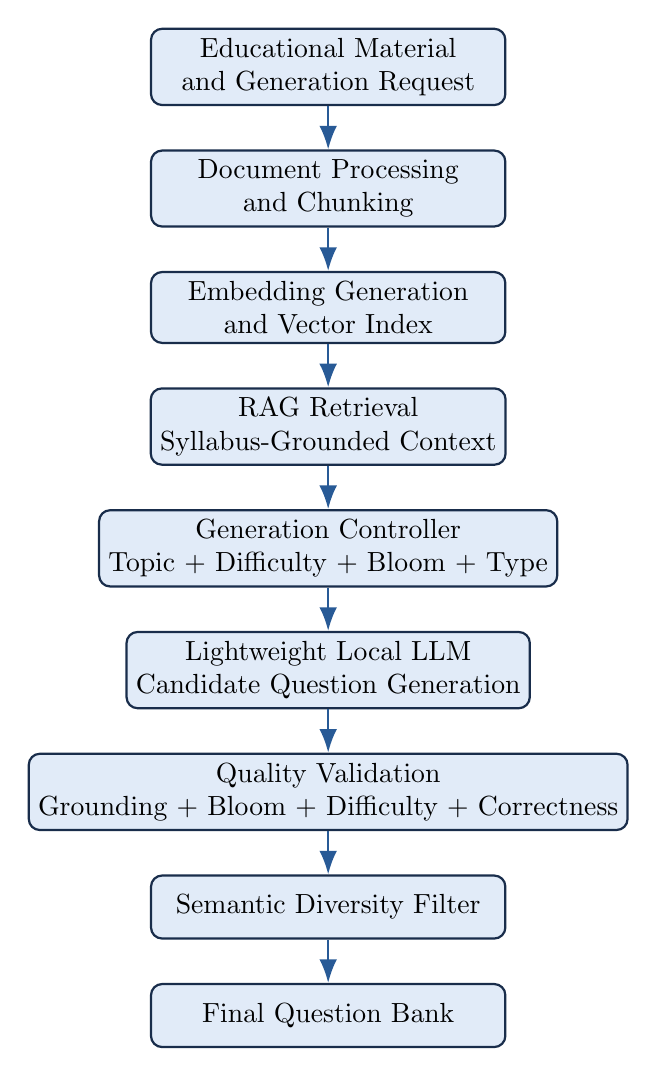
\begin{tikzpicture}[
    node distance=0.55cm,
    box/.style={
        rectangle,
        rounded corners,
        draw=navy,
        thick,
        align=center,
        minimum width=4.5cm,
        minimum height=0.8cm,
        fill=lightblue
    },
    arrow/.style={
        -{Latex[length=3mm]},
        thick,
        draw=blue
    }
]

\node[box] (input) {Educational Material\\and Generation Request};

\node[box, below=of input] (process)
{Document Processing\\and Chunking};

\node[box, below=of process] (index)
{Embedding Generation\\and Vector Index};

\node[box, below=of index] (retrieve)
{RAG Retrieval\\Syllabus-Grounded Context};

\node[box, below=of retrieve] (control)
{Generation Controller\\Topic + Difficulty + Bloom + Type};

\node[box, below=of control] (llm)
{Lightweight Local LLM\\Candidate Question Generation};

\node[box, below=of llm] (validate)
{Quality Validation\\Grounding + Bloom + Difficulty + Correctness};

\node[box, below=of validate] (diversity)
{Semantic Diversity Filter};

\node[box, below=of diversity] (output)
{Final Question Bank};

\draw[arrow] (input) -- (process);
\draw[arrow] (process) -- (index);
\draw[arrow] (index) -- (retrieve);
\draw[arrow] (retrieve) -- (control);
\draw[arrow] (control) -- (llm);
\draw[arrow] (llm) -- (validate);
\draw[arrow] (validate) -- (diversity);
\draw[arrow] (diversity) -- (output);

\end{tikzpicture}
\end{center}

\begin{figure}[H]
\centering
\caption{Proposed System Architecture}
\label{fig:architecture}
\end{figure}

\section{Layer 1: Educational Input Layer}

The system accepts:

\begin{itemize}
    \item syllabus documents;
    \item textbooks;
    \item lecture notes;
    \item reference material;
    \item subject and topic;
    \item number of questions;
    \item difficulty;
    \item Bloom's level;
    \item question type.
\end{itemize}

The user can therefore explicitly specify the desired properties of the question set.

\section{Layer 2: Document Processing}

Educational documents are processed before they become searchable.

The processing pipeline consists of:

\begin{enumerate}
    \item document extraction;
    \item text cleaning;
    \item removal of irrelevant formatting;
    \item semantic chunking;
    \item metadata assignment;
    \item embedding generation;
    \item vector indexing.
\end{enumerate}

Each chunk can contain metadata such as:

\begin{itemize}
    \item subject,
    \item unit,
    \item chapter,
    \item topic,
    \item source document,
    \item page number.
\end{itemize}

This metadata enables more precise syllabus-grounded retrieval.

\section{Layer 3: Knowledge Base and Retrieval}

The processed educational content is converted into vector representations.

Given a chunk $x$, an embedding model produces:

\[
E(x) \in \mathbb{R}^{d}
\]

where $d$ represents the embedding dimension.

For a query $q$, semantic similarity can be measured using cosine similarity:

\[
\text{sim}(q,x)
=
\frac{E(q)\cdot E(x)}
{\|E(q)\|\|E(x)\|}
\]

The top-$k$ relevant chunks are retrieved and passed to the generation stage.

\section{Layer 4: Generation Controller}

The generation controller transforms the user's request into structured constraints.

A generation request may contain:

\begin{table}[H]
\centering
\caption{Question Generation Controls}
\label{tab:controls}
\begin{tabularx}{\textwidth}{P{0.25\textwidth} Y}
\toprule
\textbf{Control} & \textbf{Possible Values}\\
\midrule
Difficulty & Easy, Medium, Hard\\
Bloom Level & Remember, Understand, Apply, Analyze, Evaluate, Create\\
Question Type & MCQ, Short Answer, Scenario-Based, Conceptual, Case-Based\\
Topic & Selected syllabus topic/subtopic\\
Grounding & Strict / Standard\\
Diversity & Similarity threshold / required diversity\\
\bottomrule
\end{tabularx}
\end{table}

The controls are applied jointly rather than independently.

For example:

\begin{quote}
Generate a hard, Analyze-level, scenario-based question from the ``Deadlock Detection'' topic using only retrieved syllabus evidence.
\end{quote}

\section{Layer 5: Retrieval-Augmented Generation}

The generation prompt is constructed from:

\[
P =
P_{\text{instruction}}
+
P_{\text{constraints}}
+
P_{\text{retrieved context}}
\]

The retrieved context acts as the grounding source.

The LLM is therefore not asked to rely solely on its pretrained knowledge.

\section{Layer 6: Candidate Question Generation}

The lightweight LLM generates a candidate set rather than immediately producing the final question bank.

For example:

\[
N_{\text{candidates}}
>
N_{\text{required}}
\]

If 10 questions are requested, the system may generate a larger candidate pool. The validation and diversity stages then select the highest-quality candidates.

\section{Layer 7: Automated Validation}

Every candidate question passes through multiple validation checks.

\subsection{Grounding Validation}

The generated question is compared with retrieved evidence.

A question is rejected if its key factual claims are unsupported by the retrieved educational material.

\subsection{Bloom-Level Validation}

The question is classified according to its expected cognitive operation.

For example:

\begin{itemize}
    \item Remember: recall a fact or definition;
    \item Understand: explain or interpret;
    \item Apply: use knowledge in a situation;
    \item Analyze: break down relationships or causes;
    \item Evaluate: judge or justify using criteria;
    \item Create: construct or design a solution.
\end{itemize}

The requested Bloom level is compared with the predicted Bloom level.

\subsection{Difficulty Validation}

Difficulty is evaluated using measurable characteristics such as:

\begin{itemize}
    \item conceptual depth;
    \item number of reasoning steps;
    \item prerequisite concepts;
    \item distractor similarity;
    \item scenario complexity.
\end{itemize}

\subsection{Answer Validation}

The generated answer is checked against the retrieved context.

For MCQs:

\[
\text{Correct Option} \in
\{\text{A},\text{B},\text{C},\text{D}\}
\]

and exactly one option should be considered correct unless the question explicitly supports multiple correct answers.

\subsection{Distractor Validation}

Distractors should:

\begin{itemize}
    \item be related to the target concept;
    \item be plausible;
    \item not be identical to the correct answer;
    \item not contain obvious formatting clues;
    \item not be completely unrelated to the question.
\end{itemize}

\section{Layer 8: Diversity Filtering}

Exact duplicate removal is insufficient.

Two questions may be different at the lexical level while testing the same concept.

Sentence embeddings are therefore used to calculate semantic similarity.

For two questions $q_i$ and $q_j$:

\[
S_{ij}
=
\cos(E(q_i),E(q_j))
\]

If:

\[
S_{ij} > \tau
\]

where $\tau$ is the configured similarity threshold, the questions are considered too similar and one candidate is removed.

This produces a final question set with greater semantic diversity.

\section{End-to-End Example}

Consider the following educational topic:

\begin{center}
\textbf{Operating Systems -- Deadlocks}
\end{center}

The requested configuration is:

\begin{itemize}
    \item Topic: Deadlock
    \item Difficulty: Hard
    \item Bloom Level: Analyze
    \item Type: Scenario-Based
    \item Grounding: Strict
\end{itemize}

The system performs:

\begin{enumerate}
    \item retrieve syllabus material related to deadlocks;
    \item identify concepts such as mutual exclusion, hold-and-wait, no preemption, and circular wait;
    \item construct a constrained generation prompt;
    \item generate candidate scenario-based questions;
    \item validate the questions against retrieved context;
    \item verify Bloom-level alignment;
    \item evaluate difficulty;
    \item validate the answer;
    \item calculate semantic similarity against accepted questions;
    \item remove repetitive candidates;
    \item add the remaining high-quality questions to the question bank.
\end{enumerate}

% ============================================================
% ALGORITHMS
% ============================================================

\section{Algorithms Used}

\subsection{Retrieval-Augmented Generation}

RAG consists of two main stages:

\begin{enumerate}
    \item retrieval of relevant educational evidence;
    \item generation using the retrieved evidence.
\end{enumerate}

\subsection{Sentence-BERT Embeddings}

Sentence-BERT is used to create semantic representations of:

\begin{itemize}
    \item educational chunks;
    \item generation queries;
    \item generated questions.
\end{itemize}

\subsection{Vector Similarity Search}

The vector index retrieves educational chunks whose semantic representations are closest to the query.

\subsection{Prompt-Based Constraint Control}

The generation controller provides structured constraints for:

\begin{itemize}
    \item topic;
    \item Bloom level;
    \item difficulty;
    \item question type;
    \item answer format;
    \item grounding requirements.
\end{itemize}

\subsection{Question Validation}

The validator operates as an acceptance gate:

\[
\text{Candidate}
\rightarrow
\begin{cases}
\text{Accept}, & \text{if constraints satisfied}\\
\text{Reject}, & \text{otherwise}
\end{cases}
\]

\subsection{Semantic Diversity Filtering}

Embedding similarity is used to identify questions that are semantically repetitive.

\subsection{Ablation Evaluation}

The system can be evaluated through progressively stronger configurations:

\[
A_0 = \text{Direct LLM}
\]

\[
A_1 = \text{Direct LLM + Controls}
\]

\[
A_2 = \text{RAG + Controls}
\]

\[
A_3 = \text{RAG + Controls + Validation}
\]

\[
A_4 = \text{RAG + Controls + Validation + Diversity}
\]

The improvement between these configurations provides evidence about the contribution of each component.

% ============================================================
% CHAPTER 8
% ============================================================

\chapter{Tools and Technology}

\section{Software Requirements}

\begin{table}[H]
\centering
\caption{Software Requirements}
\label{tab:software}
\begin{tabularx}{\textwidth}{P{0.30\textwidth} Y}
\toprule
\textbf{Technology} & \textbf{Purpose}\\
\midrule

Python 3.10+ &
Core development language for document processing, retrieval, validation, and model integration.
\\

FastAPI &
Backend API for question generation and validation services.
\\

React.js &
Frontend interface for configuring question generation.
\\

Tailwind CSS &
Frontend styling and responsive UI.
\\

PostgreSQL &
Storage of users, generation configurations, questions, validation results, and metadata.
\\

Sentence Transformers &
Generation of semantic embeddings.
\\

FAISS / ChromaDB &
Vector similarity search and retrieval.
\\

Hugging Face Transformers &
Access to embedding, classification, and lightweight language models.
\\

Ollama &
Local execution of lightweight LLMs.
\\

PyMuPDF / Document Parser &
Extraction of text from educational documents.
\\

LangChain / Custom RAG Pipeline &
Orchestration of retrieval and generation components.
\\

Git and GitHub &
Version control and collaborative development.
\\

Docker &
Reproducible deployment and service isolation.
\\

\bottomrule
\end{tabularx}
\end{table}

\section{Hardware Requirements}

\begin{table}[H]
\centering
\caption{Hardware Requirements}
\label{tab:hardware}
\begin{tabularx}{\textwidth}{P{0.30\textwidth} Y}
\toprule
\textbf{Component} & \textbf{Specification}\\
\midrule

CPU &
Intel Core i5 / AMD Ryzen 5 or better
\\

RAM &
16 GB recommended
\\

Storage &
512 GB SSD or higher
\\

GPU &
Optional; useful for faster local LLM inference
\\

Operating System &
Windows 10/11 or Linux
\\

Internet &
Required for initial package/model acquisition; local inference can operate without continuous external API access
\\

\bottomrule
\end{tabularx}
\end{table}

\section{Minimum Viable Product}

The MVP consists of:

\begin{enumerate}
    \item educational document upload;
    \item syllabus-aware document processing;
    \item vector-based retrieval;
    \item configurable topic selection;
    \item Bloom-level selection;
    \item difficulty selection;
    \item question-type selection;
    \item lightweight LLM generation;
    \item automated validation;
    \item semantic duplicate detection;
    \item final question-bank export.
\end{enumerate}

% ============================================================
% EVALUATION
% ============================================================

\chapter*{Evaluation Strategy}
\addcontentsline{toc}{chapter}{Evaluation Strategy}

The proposed system will be evaluated using both automatic metrics and human evaluation.

\section{Evaluation Dimensions}

\begin{table}[H]
\centering
\caption{Evaluation Dimensions}
\label{tab:evaluation}
\begin{tabularx}{\textwidth}{P{0.25\textwidth} Y}
\toprule
\textbf{Dimension} & \textbf{Evaluation}\\
\midrule

Syllabus Relevance &
Human rating and evidence-supported relevance score.
\\

Factual Correctness &
Comparison against retrieved source material and expert validation.
\\

Bloom Alignment &
Expert classification versus requested Bloom level.
\\

Difficulty &
Human rating and comparison between requested and perceived difficulty.
\\

Question Quality &
Expert evaluation using a structured rubric.
\\

Diversity &
Mean pairwise semantic similarity and duplicate rate.
\\

Distractor Quality &
Human evaluation of plausibility and conceptual relevance.
\\

Generation Efficiency &
Latency, memory consumption, and questions generated per unit time.
\\

\bottomrule
\end{tabularx}
\end{table}

\section{Ablation Experiment}

The key research experiment is to remove one major component at a time.

\begin{table}[H]
\centering
\caption{Ablation Configurations}
\label{tab:ablation}
\begin{tabularx}{\textwidth}{P{0.15\textwidth} P{0.55\textwidth} Y}
\toprule
\textbf{Model} & \textbf{Configuration} & \textbf{Purpose}\\
\midrule

A0 &
Direct LLM prompting &
Baseline
\\

A1 &
LLM + explicit generation controls &
Measures effect of controllability
\\

A2 &
LLM + controls + RAG &
Measures effect of syllabus grounding
\\

A3 &
RAG + controls + validation &
Measures effect of automated validation
\\

A4 &
RAG + controls + validation + diversity &
Measures complete system
\\

\bottomrule
\end{tabularx}
\end{table}

The central research question is whether the complete pipeline produces statistically and practically better questions than direct LLM prompting.

% ============================================================
% RESEARCH CONTRIBUTION
% ============================================================

\chapter*{Research Contribution}
\addcontentsline{toc}{chapter}{Research Contribution}

The project contributes a unified framework for controlled educational question generation rather than treating question generation as a single LLM inference task.

The major contributions are:

\begin{enumerate}

\item \textbf{Syllabus-grounded generation:}
Educational evidence is retrieved before generation to constrain the knowledge used by the LLM.

\item \textbf{Multi-dimensional controllability:}
Topic, difficulty, Bloom's level, question type, grounding, and diversity are jointly considered.

\item \textbf{Automated quality validation:}
Generated questions are passed through a validation layer before acceptance.

\item \textbf{Semantic diversity filtering:}
Embedding-based similarity is used to reduce repetitive questions.

\item \textbf{Lightweight deployment:}
The system is designed around models that can operate locally with modest hardware.

\item \textbf{Component-wise empirical evaluation:}
Ablation experiments quantify the contribution of RAG, controls, validation, and diversity filtering.

\end{enumerate}

% ============================================================
% BIBLIOGRAPHY
% ============================================================

\begin{thebibliography}{99}

\bibitem{elkins2024}
S. Elkins, E. Kochmar, J. C. K. Cheung, and I. Serban,
``How Teachers Can Use Large Language Models and Bloom's Taxonomy to Create Educational Quizzes,''
in \textit{Proceedings of the AAAI Conference on Artificial Intelligence}, vol. 38, 2024.

\bibitem{scaria2024}
N. Scaria, S. D. Chenna, and D. Subramani,
``How Good are Modern LLMs in Generating Relevant and High-Quality Questions at Different Bloom's Skill Levels for Indian High School Social Science Curriculum?''
in \textit{Proceedings of ACL}, 2024.

\bibitem{bloomllm2024}
N. Duong-Trung, X. Wang, and M. Kravcik,
``BloomLLM: Large Language Models Based Question Generation Combining Supervised Fine-Tuning and Bloom's Taxonomy,''
in \textit{Proceedings of EC-TEL}, 2024.

\bibitem{luo2024}
H. Luo, Y. Deng, Y. Shen, S.-K. Ng, and T.-S. Chua,
``Chain-of-Exemplar: Enhancing Distractor Generation for Multimodal Educational Question Generation,''
in \textit{Proceedings of ACL}, 2024.

\bibitem{maity2025}
S. Maity, A. Deroy, and S. Sarkar,
``Leveraging In-Context Learning and Retrieval-Augmented Generation for Automatic Question Generation in Educational Domains,''
arXiv preprint, 2025.

\bibitem{ragmcq2025}
``Retrieval-Augmented Generation for Multiple-Choice Questions and Answers Generation,''
\textit{Procedia Computer Science}, 2025.

\bibitem{pan2025}
F. Pan, Q. Zhou, W. Guo, and H. Yang,
``A Survey on Retrieval-Augmented Generation in Applications of Education and Teaching,''
\textit{Computers \& Education: Artificial Intelligence}, vol. 8, 2025.

\bibitem{schoolqg2025}
``Can Large Language Models Meet the Challenge of Generating School-Level Questions?''
\textit{Computers \& Education: Artificial Intelligence}, vol. 8, 2025.

\bibitem{ragassurvey2024}
H. Yu et al.,
``Evaluation of Retrieval-Augmented Generation: A Survey,''
arXiv preprint, 2024.

\bibitem{reimers2019}
N. Reimers and I. Gurevych,
``Sentence-BERT: Sentence Embeddings using Siamese BERT-Networks,''
in \textit{Proceedings of EMNLP-IJCNLP}, pp. 3982--3992, 2019.

\bibitem{es2024}
S. Es, J. James, L. Espinosa-Anke, and S. Schockaert,
``RAGAS: Automated Evaluation of Retrieval Augmented Generation,''
in \textit{Proceedings of EACL}, 2024.

\bibitem{lewis2020}
P. Lewis et al.,
``Retrieval-Augmented Generation for Knowledge-Intensive NLP Tasks,''
in \textit{Advances in Neural Information Processing Systems}, 2020.

\bibitem{vaswani2017}
A. Vaswani et al.,
``Attention Is All You Need,''
in \textit{Advances in Neural Information Processing Systems}, 2017.

\bibitem{devlin2019}
J. Devlin, M.-W. Chang, K. Lee, and K. Toutanova,
``BERT: Pre-training of Deep Bidirectional Transformers for Language Understanding,''
in \textit{Proceedings of NAACL-HLT}, 2019.

\bibitem{malkov2018}
Y. A. Malkov and D. A. Yashunin,
``Efficient and Robust Approximate Nearest Neighbor Search Using Hierarchical Navigable Small World Graphs,''
\textit{IEEE Transactions on Pattern Analysis and Machine Intelligence}, 2020.

\bibitem{relevance2025}
``Retrieval-Augmented Generation for Educational Applications: A Systematic Survey,''
\textit{Computers \& Education: Artificial Intelligence}, 2025.

\bibitem{distractor2024}
``Educational Question Generation and Distractor Generation with Large Language Models,''
in \textit{Proceedings of the Association for Computational Linguistics}, 2024.

\bibitem{rag2025}
``Leveraging Retrieval-Augmented Generation for Automatic Question Generation in Educational Domains,''
arXiv preprint, 2025.

\bibitem{bloom1956}
B. S. Bloom, M. D. Engelhart, E. J. Furst, W. H. Hill, and D. R. Krathwohl,
\textit{Taxonomy of Educational Objectives: The Classification of Educational Goals},
David McKay Company, 1956.

\bibitem{anderson2001}
L. W. Anderson and D. R. Krathwohl,
\textit{A Taxonomy for Learning, Teaching, and Assessing},
Longman, 2001.

\end{thebibliography}

% ============================================================
% PROGRESS SUMMARY
% ============================================================

\chapter*{Progress Summary}
\addcontentsline{toc}{chapter}{Progress Summary}

The team has completed the conceptual design of the Syllabus-Grounded Controllable Question Generation system. The project scope has been defined around automated educational question generation rather than answer evaluation or adaptive student assessment.

The team has studied recent work involving Large Language Models, Retrieval-Augmented Generation, Bloom's taxonomy, educational question generation, semantic embeddings, and automated evaluation. The literature survey indicates that existing systems demonstrate the usefulness of LLMs for question generation but leave opportunities for stronger simultaneous control, syllabus grounding, automated validation, semantic diversity, and lightweight deployment.

The system architecture has been designed around the following pipeline:

\begin{center}
\textbf{
Educational Material
$\rightarrow$
Processing
$\rightarrow$
Retrieval
$\rightarrow$
Controlled Generation
$\rightarrow$
Validation
$\rightarrow$
Diversity Filtering
$\rightarrow$
Question Bank
}
\end{center}

The proposed technology stack includes Python, FastAPI, React, PostgreSQL, Sentence Transformers, vector search, Hugging Face Transformers, and Ollama-based local LLM inference.

The next implementation stage focuses on building the document ingestion pipeline, creating the syllabus-specific vector knowledge base, integrating the generation controller, and implementing the automated validation and diversity modules.

A major research component of the project is the planned ablation study. This will compare direct LLM generation with progressively enhanced systems containing explicit controls, RAG, validation, and diversity filtering.

% ============================================================
% TEAM COLLABORATION
% ============================================================

\chapter*{Team Collaboration Evidence}
\addcontentsline{toc}{chapter}{Team Collaboration Evidence}

\section*{Student 1}

\textbf{Dhruv Gala:}

Responsible for project architecture, system planning, and integration of the question-generation pipeline. Contributed to the literature survey and formulation of the research problem.

\section*{Student 2}

\textbf{Yash Pajwani:}

Responsible for the Retrieval-Augmented Generation component, document processing, semantic chunking, embedding generation, and vector retrieval.

\section*{Student 3}

\textbf{Shravan Padhar:}

Responsible for frontend and backend development, including the question-generation interface, API integration, database management, and system deployment.

\section*{Student 4}

\textbf{Sahil Shah:}

Responsible for question validation, Bloom's taxonomy classification, difficulty analysis, semantic diversity filtering, and experimental evaluation.

% ============================================================
% FINAL PAGE
% ============================================================

\chapter*{Conclusion}
\addcontentsline{toc}{chapter}{Conclusion}

The proposed Syllabus-Grounded Controllable Question Generation system addresses the limitations of direct LLM-based educational question generation by combining retrieval, explicit controls, lightweight language models, automated validation, and semantic diversity filtering.

The central design principle is that high-quality educational question generation should not be treated as a single generation step. Instead, generation should be followed by systematic validation against the intended curriculum and educational constraints.

The planned evaluation framework further allows the project to measure whether individual components such as RAG, controllability, validation, and diversity filtering actually improve the quality of generated questions.

The resulting system aims to provide an affordable, scalable, syllabus-aware question generation framework suitable for academic institutions and resource-constrained deployment environments.

% ============================================================
% END
% ============================================================

\end{document}